\documentclass[class=book, crop=false, oneside]{standalone}
\usepackage[subpreambles=true]{standalone}

\usepackage{import}

\graphicspath{{./assets/diagrams/}}

\begin{document}

\chapter*{Translating ER into RM}
The best way to learn this mechanism is to poceed by examples.\\
Let's start with this classic:

\begin{figure}[H]
	\centering
	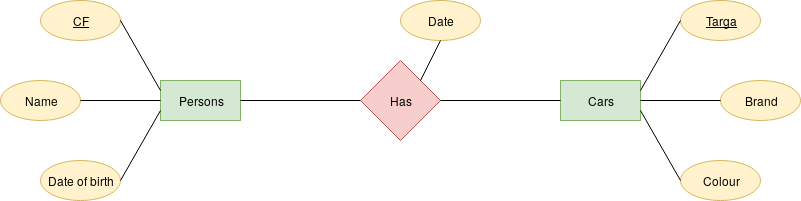
\includegraphics[width=.9\textwidth,keepaspectratio]{diagram1_00.png}
	\caption{The classic example}
	\label{diagram1.00}
\end{figure}

When we want to translate an Entity Relation Diagram (ERD) into an Relation Model (RM) we have to follow certain rules, let's check them out.
\paragraph*{Rule \#1} every entity becomes a table and its attributes are the table's columns.
\paragraph*{Rule \#2} each relation becomes a table and its attributes are part of the table's columns; also the keys of the entities involved in the relation become columns and they are flagged as Foreign Keys(FK). The FKs must be the table Key.\\
Let's put this in practice:
\vskip 20pt

\begin{minipage}{0.45\textwidth}
	PERSONS
	\begin{table}[H]
		\centering
		\subimport{assets/tables/}{phc-pers.tex}
	\end{table}
	\texttt{PERSONS(\underline{CF}, Name, Birth date)}
\end{minipage}
\hspace{.1\textwidth}
\begin{minipage}{.45\textwidth}
	CARS
	\begin{table}[H]
		\centering
		\subimport{assets/tables/}{phc-cars}
	\end{table}
	\texttt{CARS(\underline{Targa}, Brand, Color)}
\end{minipage}
\vskip 20pt
That was pretty easy, wasn't it?\\
Now it's time to draw the relation table:
\vskip 20pt
\begin{minipage}{.7\textwidth}
	HAS
	\begin{table}[H]
		\subimport{assets/tables/}{phc-has}
		\texttt{HAS(\underline{CF} \underline{Targa}, Date)}
	\end{table}
\end{minipage}
\vskip 20pt
Well, that's clear. Now it's time to mix up things a little bit.
What if we want that a car can't be owned by different people? (see \ref{diagram1.01})
\begin{figure}[H]
	\centering
	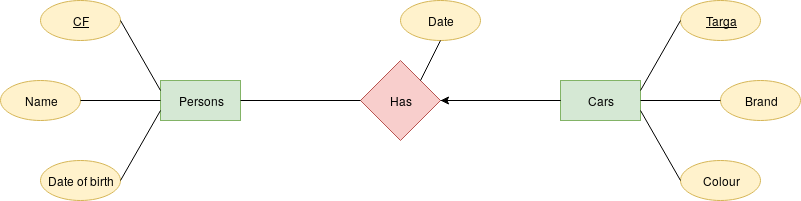
\includegraphics[width=.9\textwidth,keepaspectratio]{diagram1_01.png}
	\caption{A car now can have at most one owner}
	\label{diagram1.01}
\end{figure}
We must use only the Targa as key in Has relation.
% TODO inserire qua una tabella con la rappresentazione di ciò??
\\
And what if we want the car to have also at least one owner? (see \ref{diagram1_02})
\begin{figure}[H]
	\centering
	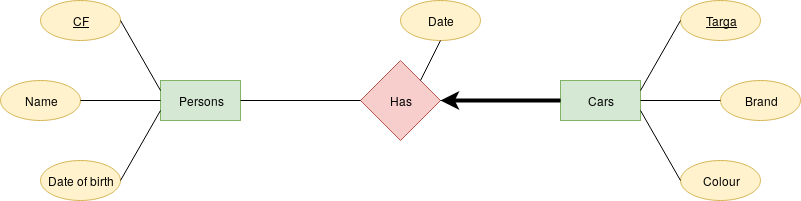
\includegraphics[width=.9\textwidth,keepaspectratio]{diagram1_02.png}
	\caption{A car now can have at most one owner}
	\label{diagram1_02}
\end{figure}
Now that a car must be owned by one person it has no more sense to keep HAS table and CARS table divided: the wittest solution is to delete HAS table and introduce in CARS table two columns, one for Date and one for CF, which will be a FK. Last but not least the CF field must be mapped as not-null.
That's the representation in RM:
\vskip 20pt
\begin{minipage}{.8\textwidth}
	CARS
	\begin{table}[H]

		\subimport{assets/tables/}{phc-cars_v2}
		\texttt{CARS(\underline{Targa}, Brand, Color, CF, Date)}
		\\CF not null
		\\CF Foreign Key to PERSONS
	\end{table}
\end{minipage}


% \begin{minipage}{\textwidth}
% 	\vskip 20pt
%
% 	\begin{minipage}{\textwidth}
%
% 		\begin{table}[H]
% 			\centering
% 			\subimport{assets/tables/}{phc-cars_v2}
% 		\end{table}
%
% 	\end{minipage}



\end{document}
